\begin{comment}
\begin{frame}[fragile]{\boss{Extra Exercise}}
	There are four extra exercises for you to practice what have learned in normalisation lecture. 
	As normalisation is one of the most challenging parts of the fundamental database module, it would be helpful for you to evaluate your understanding of this part. \\
\end{frame}
\end{comment}

\begin{frame}[fragile]{\boss{Extra} - Case 1}
	We are designing a warehouse management system for a lot of warehouses. Each warehouse ($W$) has one manager ($M$), and each manager only manage one warehouse. There could be many products ($P$) in per warehouse. For each product we also record its stock number ($S$).\\\vspace{10pt}
	\textbf{Questions}:\\
	(1) Find \textbf{candidate key(s)} and \textbf{prime attribute(s)} from attribute closures $\Sigma^{+}$.\\
	(2) Compute the \textbf{compact minimal cover} of $R$ with all FDs $\Sigma$.\\
	(3) Determine if it is \textbf{2NF}? If yes, is it \textbf{3NF}? If yes, is it \textbf{BCNF}?\\
	(4) If it is not 3NF, \textbf{synthesis} the relations to make it 3NF.\\
	(5) If it is not BCNF, \textbf{decomposite} the relations to make it BCNF and verify the \textbf{dependency preservation}. 
\end{frame}

\begin{frame}[fragile]{\boss{Extra} - Case 2}
	We are designing a transcript issuing system for our university. 
	Each student is identified by its matric number/student ID, written as $S$.
	We are going to record a grade ($G$) for each student ($S$) and each module ($M$).
	We also record students' names ($N$) and their faculty ($F$). In case any verification is needed, we also save the dean's name for each department ($D$) so that people can contact him/her.\\\vspace{10pt}
	\textbf{Questions}:\\
	(1) Find \textbf{candidate key(s)} and \textbf{prime attribute(s)} from attribute closures $\Sigma^{+}$.\\
	(2) Compute the \textbf{compact minimal cover} of $R$ with all FDs $\Sigma$.\\
	(3) Determine if it is \textbf{2NF}? If yes, is it \textbf{3NF}? If yes, is it \textbf{BCNF}?\\
	(4) If it is not 3NF, \textbf{synthesis} the relations to make it 3NF.\\
	(5) If it is not BCNF, \textbf{decomposite} the relations to make it BCNF and verify the \textbf{dependency preservation}. 
\end{frame}

\begin{frame}[fragile]{\boss{Extra} - Case 3}
	This time we deal with abstract relations with functional dependencies shown as in the figure below:\\\vspace{-5pt}
	
	\begin{figure}
		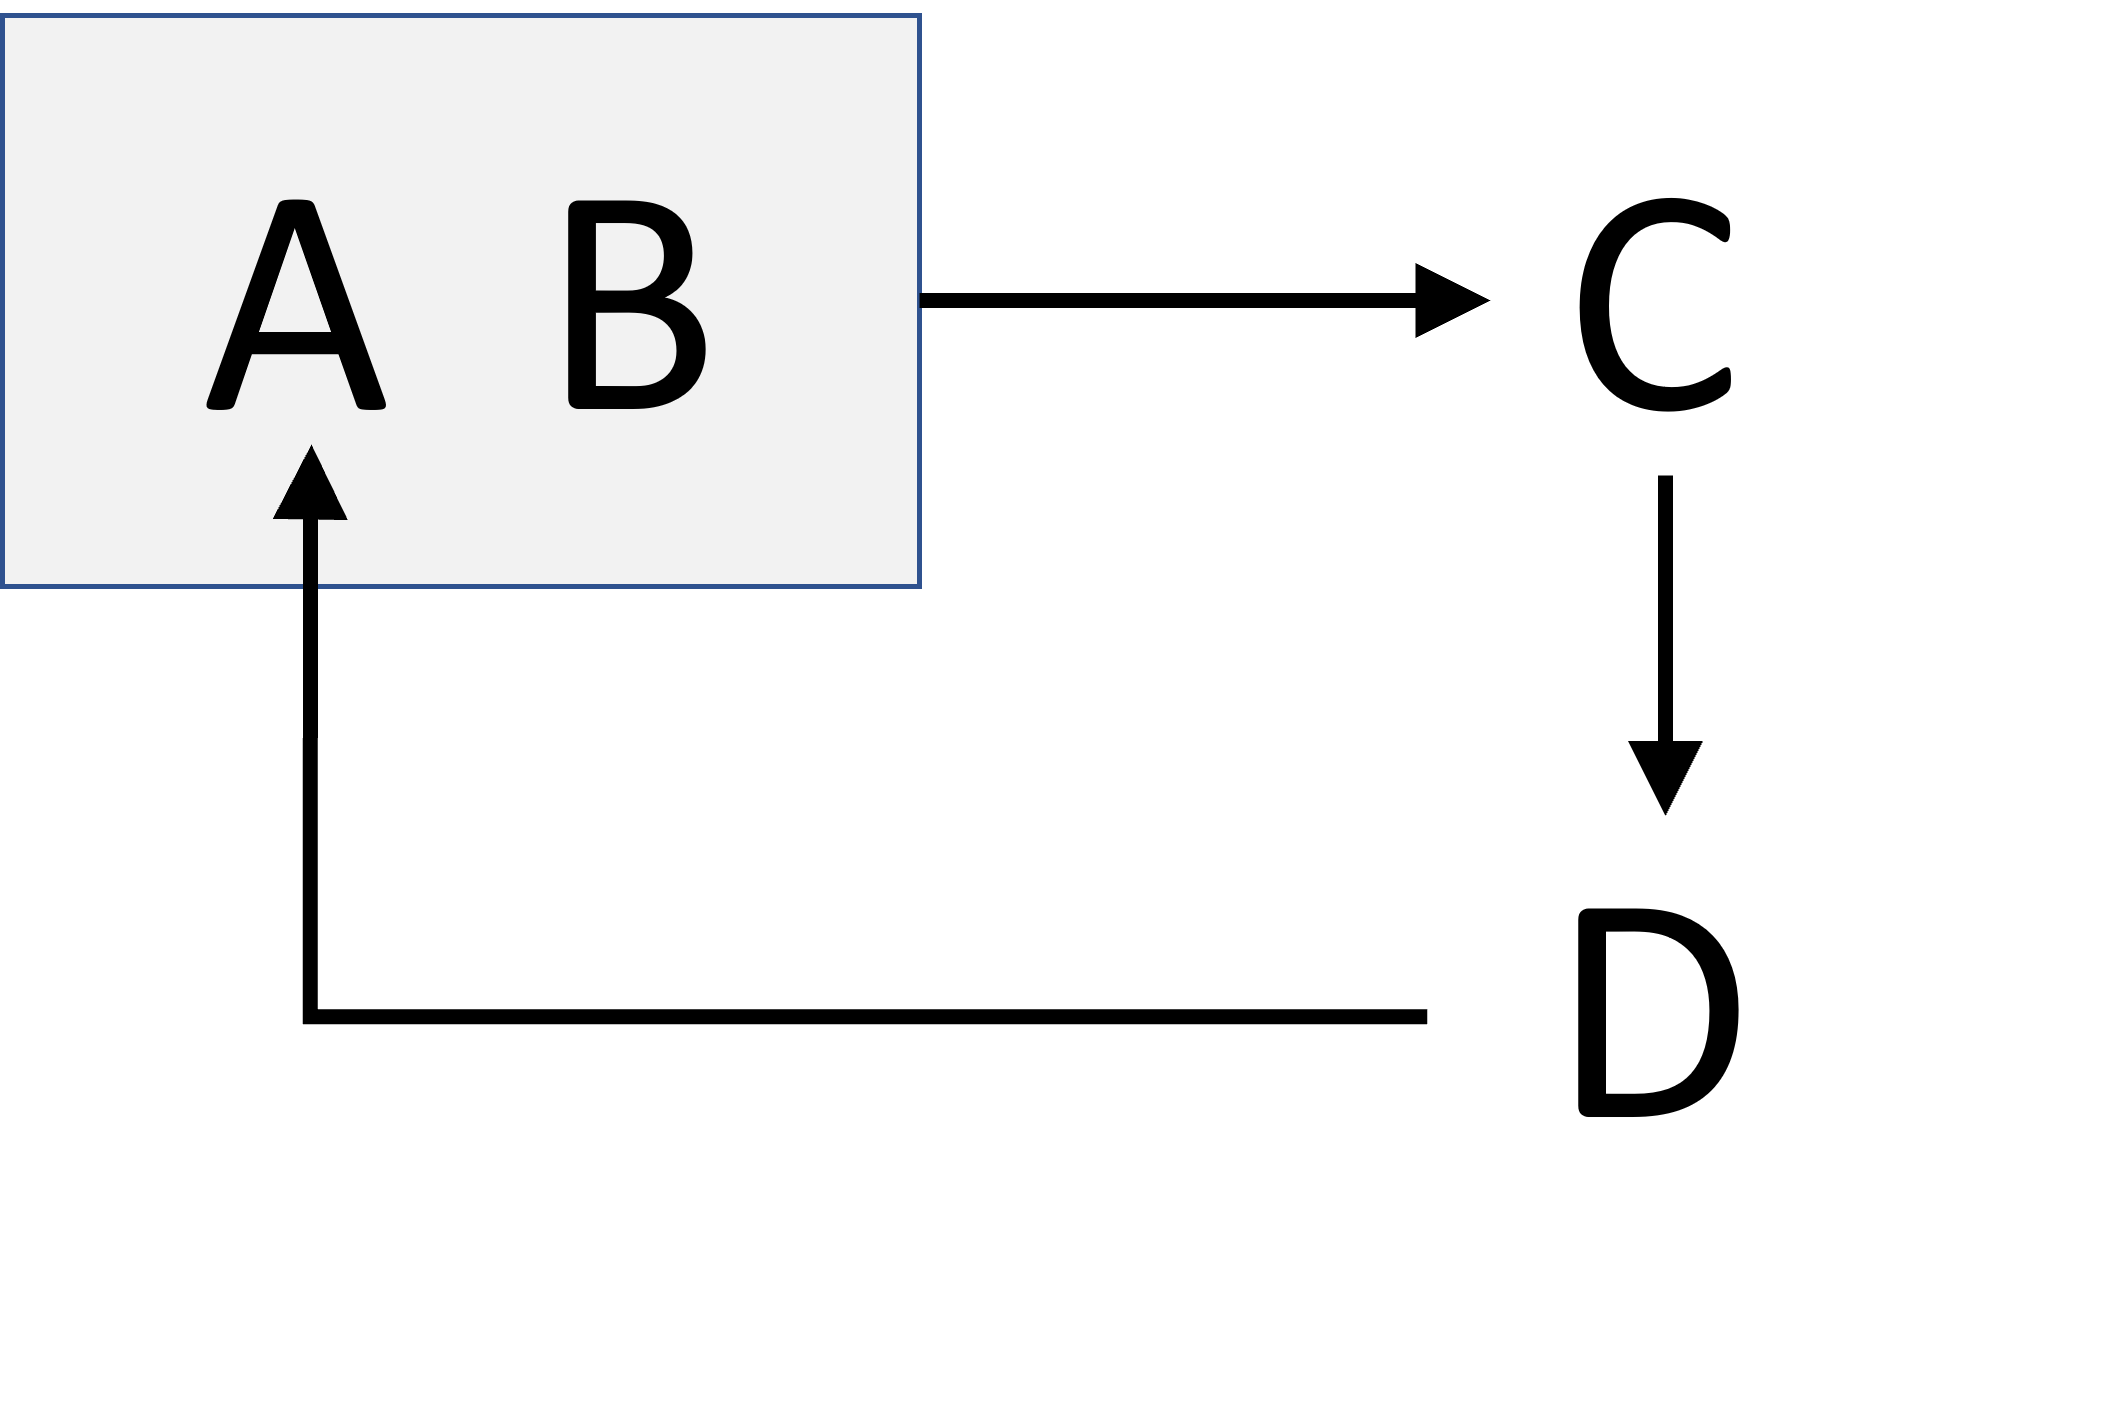
\includegraphics[width=0.4\textwidth, trim=0 0 0 0, clip]{t5/images/case3.png}
	\end{figure}\vspace{-10pt}
	
	\textbf{Questions}:\\
	(1) Find \textbf{candidate key(s)} and \textbf{prime attribute(s)} from attribute closures $\Sigma^{+}$.\\
	(2) Compute the \textbf{compact minimal cover} of $R$ with all FDs $\Sigma$.\\
	(3) Determine if it is \textbf{2NF}? If yes, is it \textbf{3NF}? If yes, is it \textbf{BCNF}?\\
	(4) If it is not 3NF, \textbf{synthesis} the relations to make it 3NF.\\
	(5) If it is not BCNF, \textbf{decomposite} the relations to make it BCNF and verify the \textbf{dependency preservation}. 
\end{frame}

\begin{frame}[fragile]{\boss{Extra} - Case 4}
	Another abstract relations with functional dependencies shown as in the figure below:\\\vspace{-5pt}
	
	\begin{figure}
		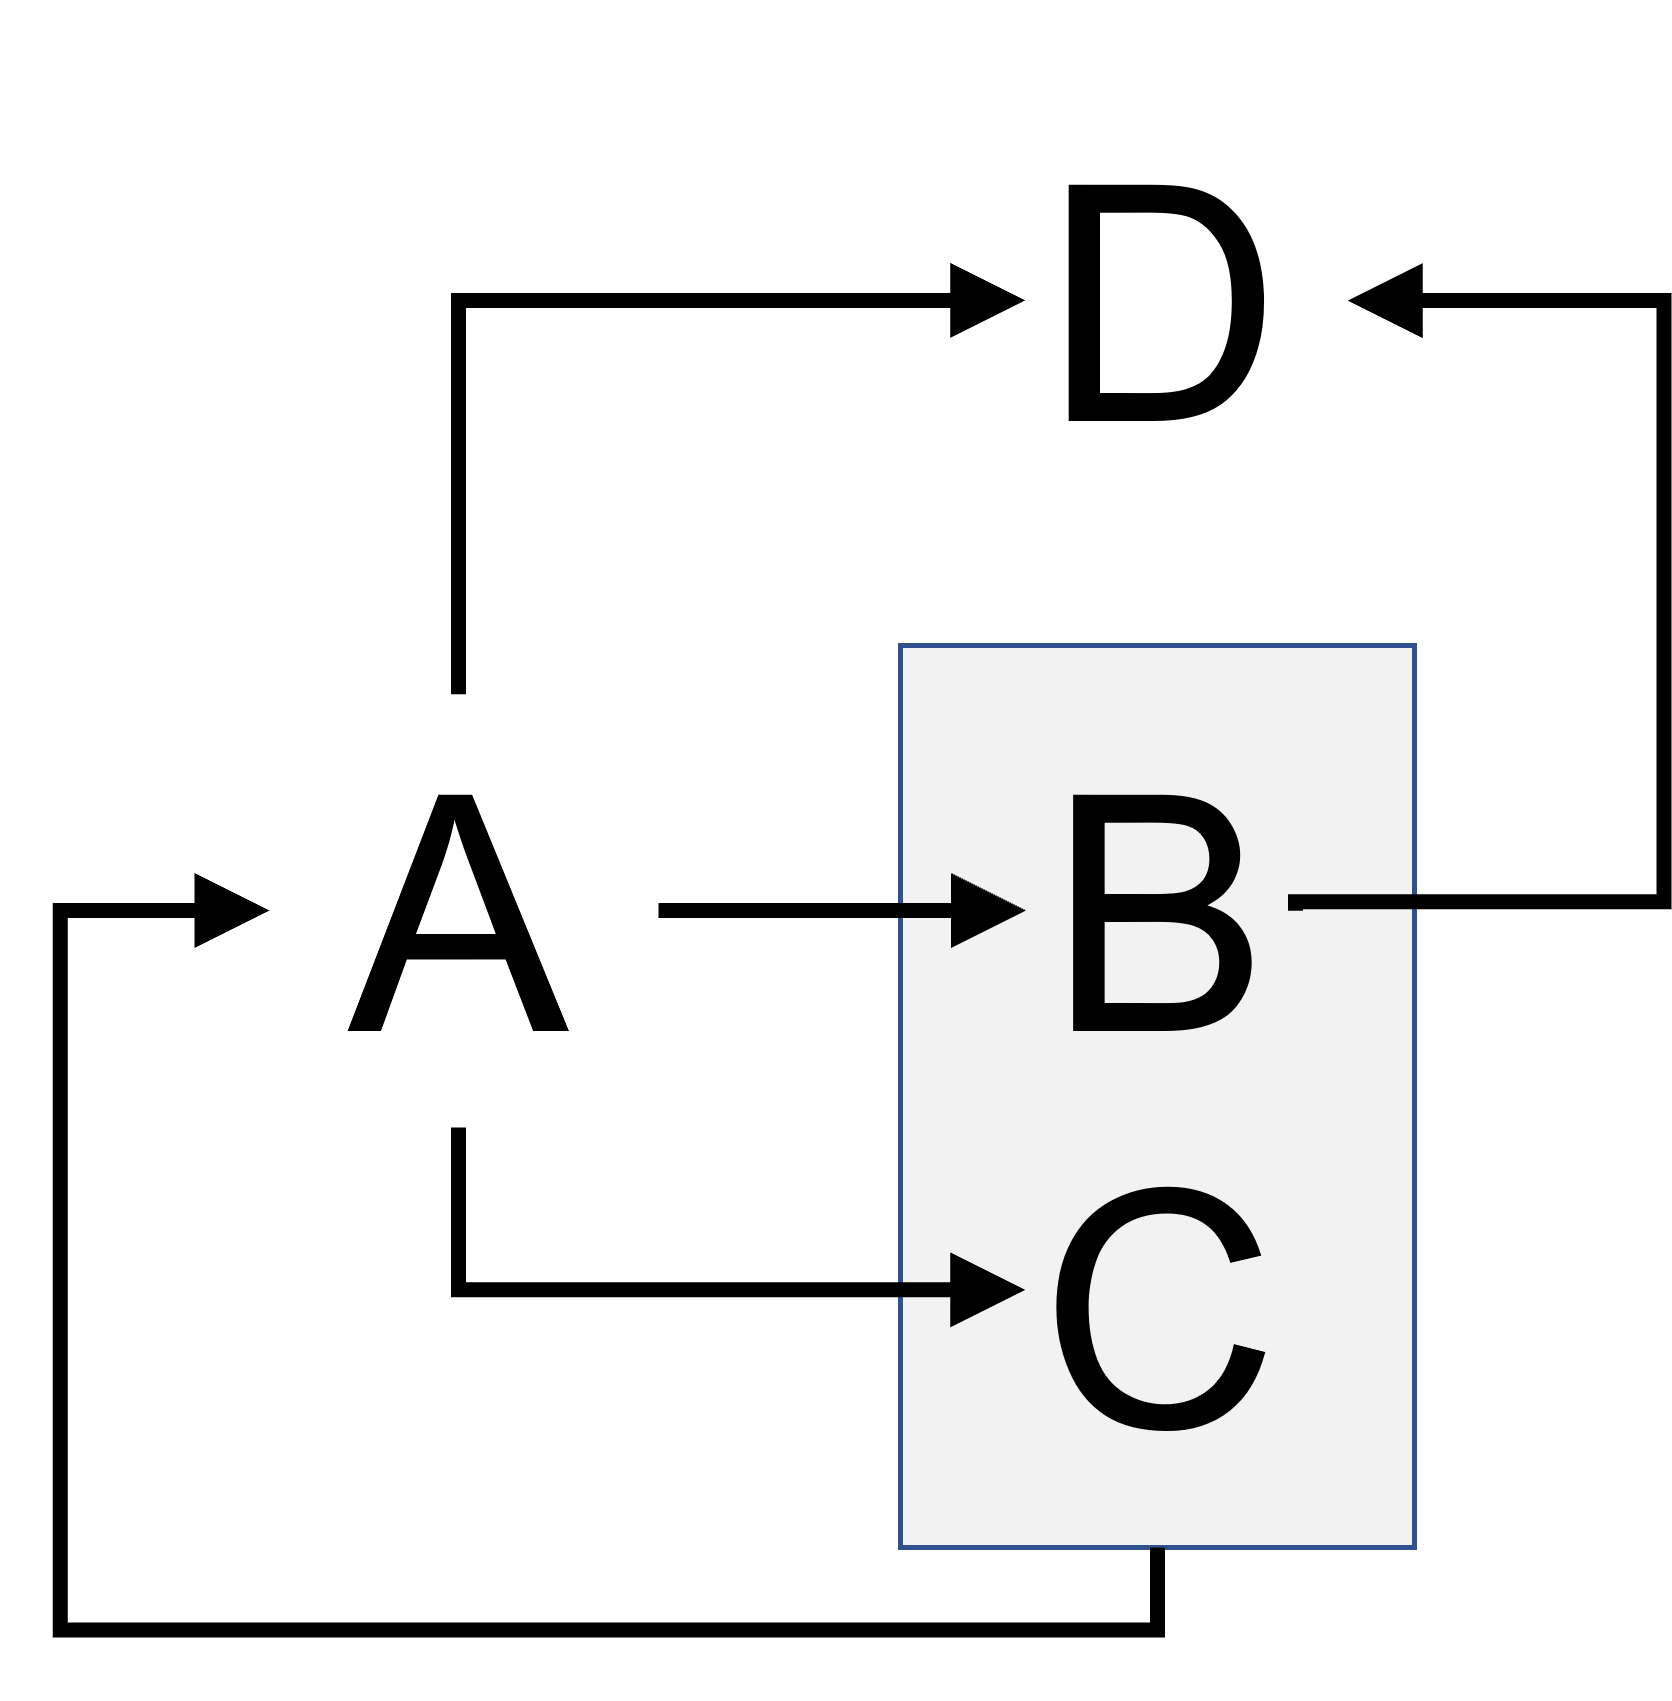
\includegraphics[width=0.25\textwidth, trim=0 0 0 0, clip]{t5/images/case4.png}
	\end{figure}\vspace{-5pt}
	
	\textbf{Questions}:\\
	(1) Find \textbf{candidate key(s)} and \textbf{prime attribute(s)} from attribute closures $\Sigma^{+}$.\\
	(2) Compute the \textbf{compact minimal cover} of $R$ with all FDs $\Sigma$.\\
	(3) Determine if it is \textbf{2NF}? If yes, is it \textbf{3NF}? If yes, is it \textbf{BCNF}?\\
	(4) If it is not 3NF, \textbf{synthesis} the relations to make it 3NF.\\
	(5) If it is not BCNF, \textbf{decomposite} the relations to make it BCNF and verify the \textbf{dependency preservation}. 
\end{frame}

